%!TEX root = ../../main.tex

\section{The AIGER format}

This section presents an important format highly used in model checking and reactive synthesis: AIGER. 

The AIGER format is used to describe circuits by multi-rooted And-Inverter Graphs (AIG) with latches that store the system state. It was developed as a compact and simple file format benchmarks for the hardware model checking competition (HWMCC). 
A And-Inverter Graph is a directed, acyclic graph that represents a structural implementation of the logical functionality of a circuit or network. An AIG consists of two-input nodes representing logical conjunction, terminal nodes labeled with variable names and edges optionally containing markers indicating logical negation. This representation of a logic function is rarely structurally efficient for large circuits, but is an efficient representation for the manipulation of Boolean functions.
Conversion from the network of logic gates to AIGs is fast and scalable. It only requires that every gate be expressed in terms of AND and NOT gates.
This conversion does not lead to unpredictable increase in memory use and runtime. This makes AIG an efficient representation in comparison with either the binary decision diagram (BDD) or the sum-of-product ($\Sigma o \Pi$) form.

% TODO: example of aig?

A file in AIGER format (ASCII variant) consists of the following parts: header, input definitions, latch definitions, output definitions and and-gate definitions. The header consists of a single line \lstinline{aag M I L O A}, where \lstinline{M} gives the maximum variable index, \lstinline{I} the number of inputs, \lstinline{L} the number of latches, \lstinline{O} the number of outputs and \lstinline{A} the number of AND gates.
Boolean variables are referred by even numbers, while odd numbers are referred to the negation of a variable, i.e. if $n$ is even, $n+1$ is the negation of $n$. $0$ and $1$ are special indexes referring the false and true values, respectively.
Then, the format can be divided in 5 sections declared in the header.

\begin{lstlisting}[caption=The empty circuit without inputs nor outputs and constant false/true in AIGER format]
aag 0 0 0 0 0             header

aag 0 0 0 1 0             header
    0                     output

aag 0 0 0 1 0             header
    1                     output
\end{lstlisting}

Every input definition takes one line and consists of a single even number.
Every latch definition takes one line and consists of an even number, followed by a number that defines which variable is used to update the latch in every step. The initial value is given by an additional number between either 0, 1 or the latch itself, which means to set the initial value to false, true or undefined, respectively. By default latches are assumed to have initial value 0.
Every output definition takes one line and consists of a single number, representing a possibly negated input, latch or and-gate. 
Every and-gate definition takes one line and consists of three numbers. The first is an even number, representing the output of the and-gate, and is followed by two numbers representing its (possibly negated) inputs.
There are also two further optional sections: symbol table and comments. The symbol table assigns names to inputs, latches and outputs. It is optional, and need not be complete. Every line defines the name of one input, latch, or output, and starts with i, l, o, respectively,
followed by the number of the input, latch, or output in the sequence of definitions.

As notable example we want to show how to encode a full-adder in AIGER format. A full-adder needs no presentation, it is just a circuits which sum two bits considering the carry.
Usually, a full-adder has three inputs: the two addends and the carry of the previous sum. That's because a full-adder is designed to be chained to other full-adders in order to sum sequence of bits. 
The first full-adder has carry value set to false, while the $i$ full-adder has the carry value in input set to the $i-1$ full-adder carry output. 
In our example, the full-adder is designed to be used as a stand-alone circuit where the carry result is saved in a latch and is used in the next computation, and it is $0$ initially.
Basically, this design choice was made just to show how to encode latches in AIGER format.

\begin{figure}[!htp]
    \centering
    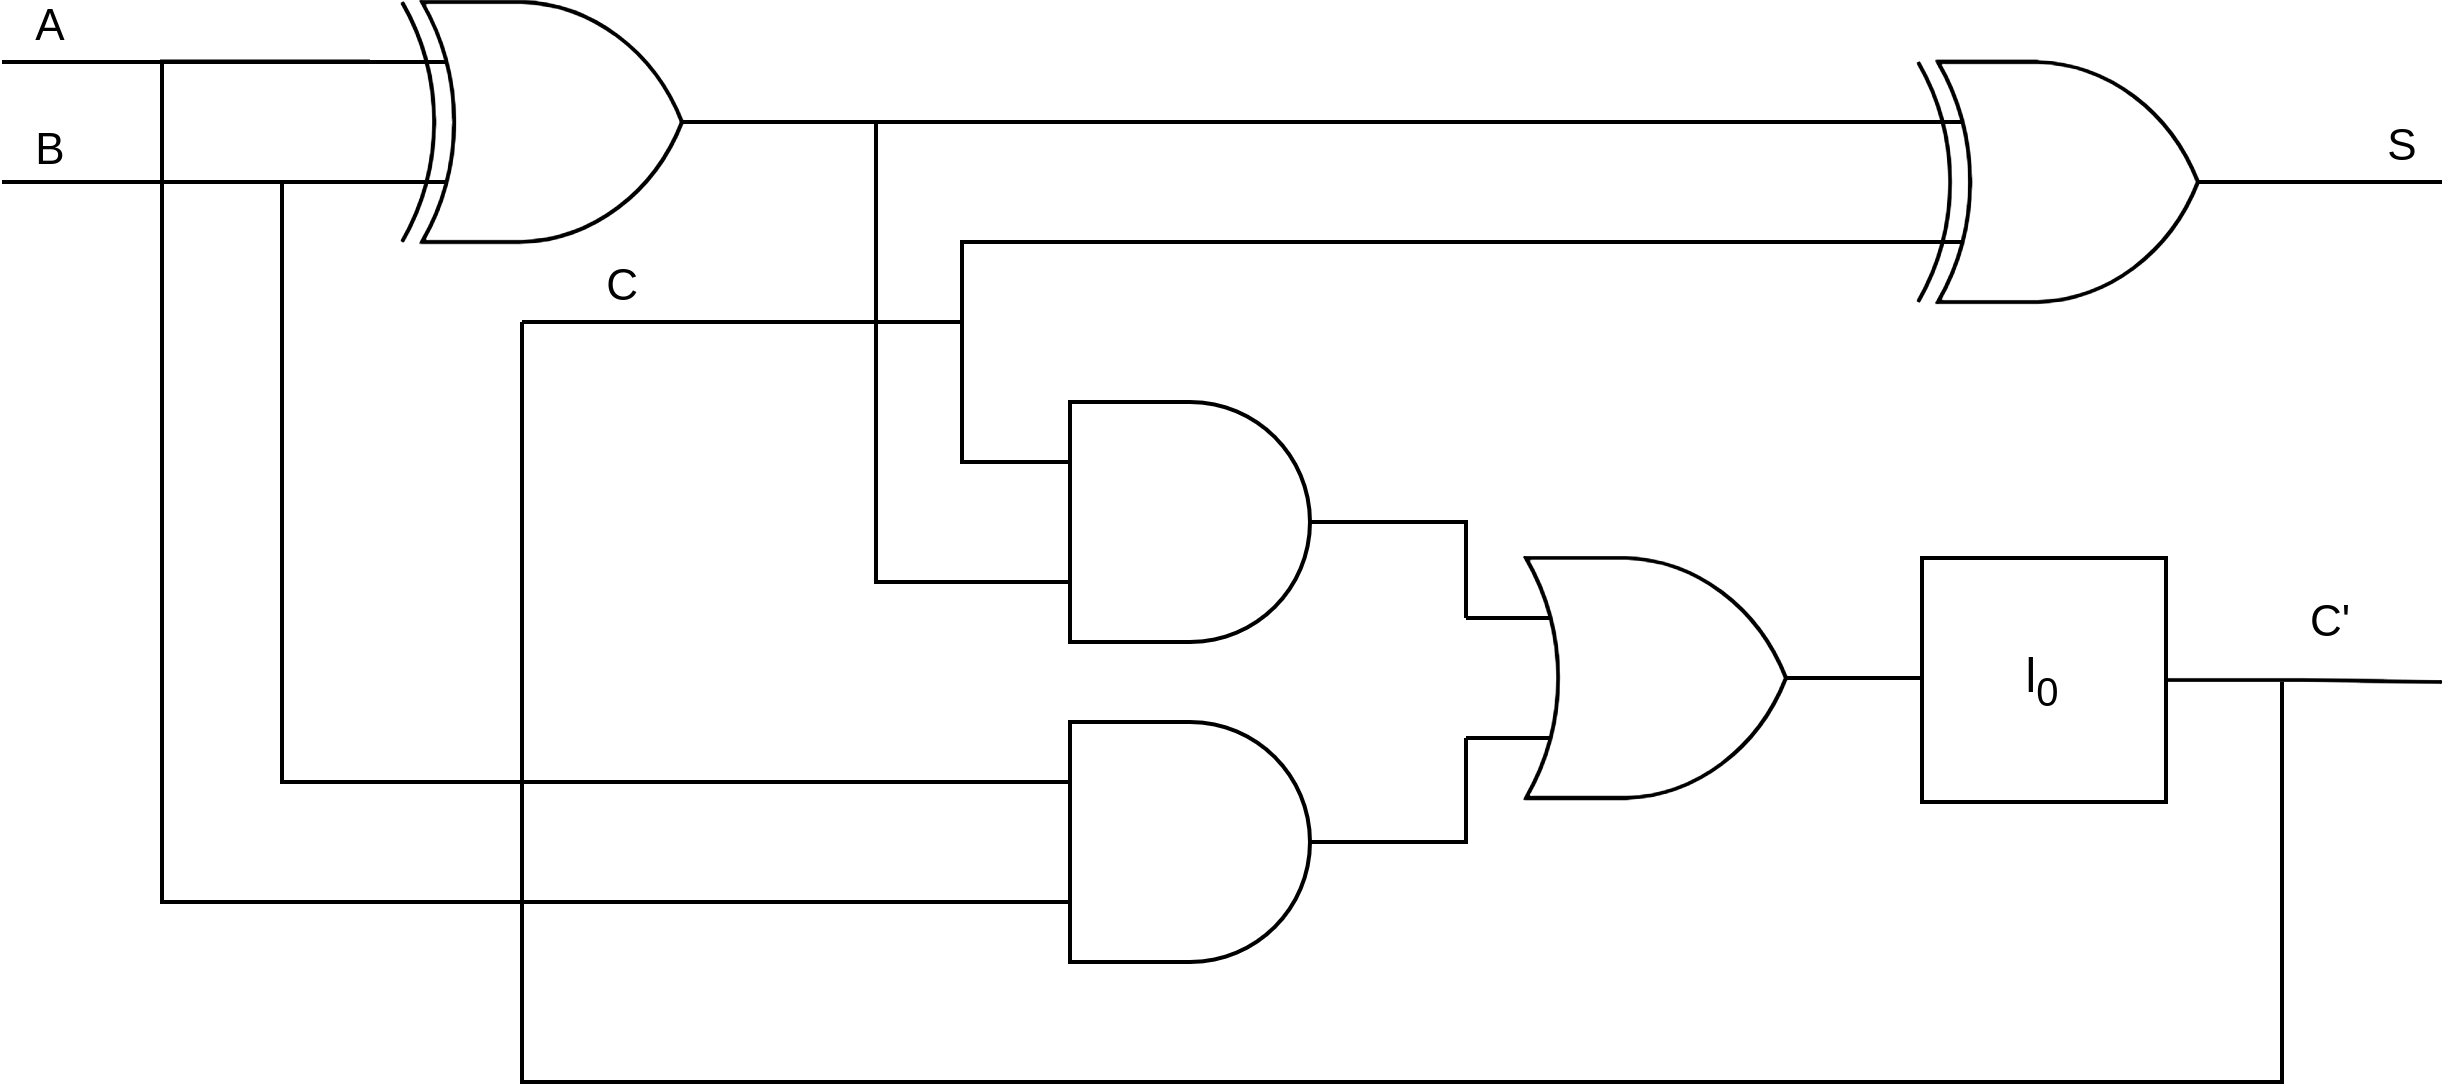
\includegraphics[width=0.6\linewidth]{figures/full-adder-circuit.png}
    \caption{Full adder circuit}
    \label{fig:full-adder-circuit}
\end{figure}

To encode a full-adder we have to express two formulas by just using and and not gates: the sum result and the carry result.
The sum result is given by $S = (A \oplus B) \oplus C$, while the carry result $C' = (A \land B) \lor (C \land (A \oplus B))$. $A$, $B$ are the input bits and $C$ the carry value.
The first step is to convert the formula to Conjunctive Normal Form (CNF) and then remove the or gates by De Morgan's laws. 

\begin{figure}
    \centering
\begin{flalign*}
& (A \oplus B) \oplus C \\
& \iff \text{(by CNF)} \\
& (\neg A \lor \neg B \lor C) \land (\neg A \lor B \lor \neg C) \land (A \lor \neg B \lor \neg C) \land (A \lor B \lor C) \\
& \iff \text{(by De morgan's laws)} \\
& \neg(A \land B \land \neg C) \land \neg(A \land \neg B \land C) \land \neg(\neg A \land B \land C) \land \neg(\neg A \land \neg B \land \neg C)
\end{flalign*}
    \caption{Expressing full-adder sum result via $\land$ and $\neg$ gates}
\end{figure}

\begin{figure}[!htp]
    \centering
    \begin{flalign*}
    & (A \land B) \lor (C \land (A \oplus B)) \\
    & \iff \text{(by CNF)} \\
    & (A \lor B) \land (A \lor C) \land (B \lor C) \\
    & \iff \text{(by De Morgan's laws)} \\
    & \neg(\neg A \land \neg B) \land \neg(\neg A \land \neg C) \land \neg(\neg B \land \neg C)
    \end{flalign*}
    \caption{Expressing full-adder carry result via $\land$ and $\neg$ gates}
\end{figure}

\begin{lstlisting}[caption = Full-adder in AIGER format]
agg 19 2 1 2 16
    2             input A
    4             input B
    6 14          latch C
    38            output sum
    16            output carry
    -- carry result
    8  3  5       !A & !B
    10 3  7       !A & !C
    12 5  7       !B & !C
    14 9  11      !(!A & !B) & !(!A & !C)
    16 14 13      !(!A & !B) & !(!A & !C) & !(!B & !C)
    -- sum result
    18 2  4       A & B
    20 18 7       A & B & !C
    22 2  5       A & !B
    24 22 6       A & !B & C
    26 3  4       !A & B
    28 26 6       !A & B  & C
    30 3  5       !A & !B 
    32 30 7       !A & !B & !C
    34 21 25      !(A & B & !C) & !(A & !B & C)
    36 34 29      !(A & B & !C) & !(A & !B & C) & !(!A & B & C)
    38 36 33      !(A & B & !C) & !(A & !B & C) & !(!A & B & C) & !(!A & !B & !C)
    i0 A
    i1 B
    o0 sum
    o1 carry
    Full adder in AIGER format
\end{lstlisting}

The usual AIGER format can not cope with reactive synthesis, so in \cite{jacobs2014extended} has been proposed an extended AIGER format for controller synthesis. They suggest to reserve the special string \lstinline{controllable_} and pretend it to the names of controllable input variables. 
All other input variables are implicitly controlled by the environment.
